\documentclass[border=1.5pt]{standalone}
\usepackage{amsmath,amssymb}
\usepackage{tikz}
\usetikzlibrary{arrows.meta,calc,positioning,shapes,shapes.misc,shapes.geometric,backgrounds,fit,decorations.pathreplacing,quantikz2}
% Shared colors and styles for the XYZ^2 figures.
% Pauli types: bright tones for fills and bands, deep (800) shades of the same hues for labels.
% The label shades keep the hue of each Pauli, are well separated from each other (CIEDE2000 > 20)
% and have a contrast ratio of at least 2.9 on the coral cells and 4.5 on the sunflower cells.
\definecolor{PauliX}{HTML}{F97316}
\definecolor{PauliY}{HTML}{EC4899}
\definecolor{PauliZ}{HTML}{9333EA}
\definecolor{PauliXText}{HTML}{AC340B}
\definecolor{PauliYText}{HTML}{9D174D}
\definecolor{PauliZText}{HTML}{5B21B6}
% Generator classes: S0 (class B, even links, coral) and gauge (class A, odd links, sunflower)
\definecolor{Szero}{HTML}{F0435E}
\definecolor{SzeroText}{HTML}{BE123C}
\definecolor{Gauge}{HTML}{F59E0B}
\definecolor{GaugeText}{HTML}{B45309}
\colorlet{GaugeGray}{Gauge}
\definecolor{ClassB}{HTML}{FF8A99}
\definecolor{ClassA}{HTML}{FFD23F}
% Logical operators (X-bar violet, Z-bar crimson), errors, ink
\definecolor{LogicalZ}{HTML}{E11D48}
\definecolor{LogicalGold}{HTML}{7C3AED}
\definecolor{ErrRed}{HTML}{1C1917}
\definecolor{InkDark}{HTML}{292524}
\definecolor{InkSoft}{HTML}{57534E}
% Labels drawn on top of colored cells
\colorlet{CellText}{InkDark}
% Noise channels
\definecolor{ErrFlip}{HTML}{EF4444}
\definecolor{Idle}{HTML}{EC4899}
\definecolor{TwoQ}{HTML}{7C3AED}
% Protocol steps
\definecolor{StepPrep}{HTML}{F97316}
\definecolor{StepMeas}{HTML}{D946EF}
\definecolor{StepDec}{HTML}{7C3AED}
\definecolor{StepRec}{HTML}{DB2777}
\tikzset{
  qb/.style={circle, draw=InkDark, line width=0.6pt, fill=white,
             minimum size=4.2mm, inner sep=0pt, font=\scriptsize},
  qbsmall/.style={circle, draw=InkDark, line width=0.5pt, fill=white,
             minimum size=2.6mm, inner sep=0pt},
  hexedge/.style={line width=0.65pt, draw=InkSoft},
  linkedge/.style={line width=1.6pt, draw=InkDark},
  bndedge/.style={line width=0.65pt, draw=InkSoft, densely dashed},
  plabel/.style={font=\scriptsize\bfseries, inner sep=1pt},
  panel/.style={font=\small\bfseries, anchor=north west},
}

\providecommand{\ket}[1]{\left|#1\right\rangle}

\begin{document}
\setlength{\tabcolsep}{0pt}
\begin{tabular}{@{}l@{}}
\textbf{(a)}\\[-6pt]
\hspace{3mm}
\begin{quantikz}[row sep={0.4cm,between origins}, column sep=0.22cm]
\setwiretype{n} & \scriptsize\textcolor{InkSoft}{1} & \scriptsize\textcolor{InkSoft}{2} & \scriptsize\textcolor{InkSoft}{3} & \scriptsize\textcolor{InkSoft}{4} & \scriptsize\textcolor{InkSoft}{5} & \scriptsize\textcolor{InkSoft}{6} & \\
\lstick{\footnotesize ancilla $\ket{+}$} & \ctrl{1} & \ctrl{6} & \ctrl{2} & \ctrl{5} & \ctrl{3} & \ctrl{4} & \meter[style={fill=PauliX!25, draw=PauliX, line width=0.7pt}]{\textcolor{PauliXText}{\boldsymbol{X}}} \\
\lstick{\footnotesize top} & \gate[style={fill=PauliX!35, draw=PauliX, line width=0.7pt}]{\textcolor{PauliXText}{\boldsymbol{X}}} & & & & & & \\
\lstick{\footnotesize upper right} & & & \gate[style={fill=PauliY!35, draw=PauliY, line width=0.7pt}]{\textcolor{PauliYText}{\boldsymbol{Y}}} & & & & \\
\lstick{\footnotesize lower right} & & & & & \gate[style={fill=PauliZ!35, draw=PauliZ, line width=0.7pt}]{\textcolor{PauliZText}{\boldsymbol{Z}}} & & \\
\lstick{\footnotesize bottom} & & & & & & \gate[style={fill=PauliX!35, draw=PauliX, line width=0.7pt}]{\textcolor{PauliXText}{\boldsymbol{X}}} & \\
\lstick{\footnotesize lower left} & & & & \gate[style={fill=PauliY!35, draw=PauliY, line width=0.7pt}]{\textcolor{PauliYText}{\boldsymbol{Y}}} & & & \\
\lstick{\footnotesize upper left} & & \gate[style={fill=PauliZ!35, draw=PauliZ, line width=0.7pt}]{\textcolor{PauliZText}{\boldsymbol{Z}}} & & & & &
\end{quantikz}\\[2pt]
\begin{tabular}{@{}lllll@{}}
\textbf{(b)} & \textbf{(c)} & & & \textbf{(d)}\\
\raisebox{-0.5\height}{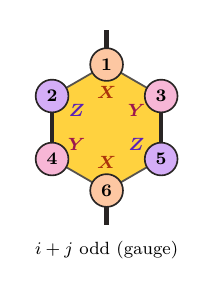
\begin{tikzpicture}[scale=0.8, every node/.style={transform shape}]
\fill[ClassA] (0.000,1.000) -- (0.866,0.500) -- (0.866,-0.500) -- (0.000,-1.000) -- (-0.866,-0.500) -- (-0.866,0.500) -- cycle;
\draw[hexedge] (0.000,1.000) -- (0.866,0.500) -- (0.866,-0.500) -- (0.000,-1.000) -- (-0.866,-0.500) -- (-0.866,0.500) -- cycle;
\draw[linkedge] (0.866,0.500) -- (0.866,-0.500);
\draw[linkedge] (-0.866,0.500) -- (-0.866,-0.500);
\draw[linkedge] (0,1.000) -- (0,1.550);
\draw[linkedge] (0,-1.000) -- (0,-1.550);
\node[qb, fill=PauliX!40, minimum size=5.2mm, font=\footnotesize\bfseries] at (0.000,1.000) {1};
\node[plabel, text=PauliXText, font=\footnotesize] at (0.000,0.550) {$\boldsymbol{X}$};
\node[qb, fill=PauliY!40, minimum size=5.2mm, font=\footnotesize\bfseries] at (0.866,0.500) {3};
\node[plabel, text=PauliYText, font=\footnotesize] at (0.476,0.275) {$\boldsymbol{Y}$};
\node[qb, fill=PauliZ!40, minimum size=5.2mm, font=\footnotesize\bfseries] at (0.866,-0.500) {5};
\node[plabel, text=PauliZText, font=\footnotesize] at (0.476,-0.275) {$\boldsymbol{Z}$};
\node[qb, fill=PauliX!40, minimum size=5.2mm, font=\footnotesize\bfseries] at (0.000,-1.000) {6};
\node[plabel, text=PauliXText, font=\footnotesize] at (0.000,-0.550) {$\boldsymbol{X}$};
\node[qb, fill=PauliY!40, minimum size=5.2mm, font=\footnotesize\bfseries] at (-0.866,-0.500) {4};
\node[plabel, text=PauliYText, font=\footnotesize] at (-0.476,-0.275) {$\boldsymbol{Y}$};
\node[qb, fill=PauliZ!40, minimum size=5.2mm, font=\footnotesize\bfseries] at (-0.866,0.500) {2};
\node[plabel, text=PauliZText, font=\footnotesize] at (-0.476,0.275) {$\boldsymbol{Z}$};
\node[font=\footnotesize, align=center] at (0,-1.950) {$i+j$ odd (gauge)};
\end{tikzpicture}} & \raisebox{-0.5\height}{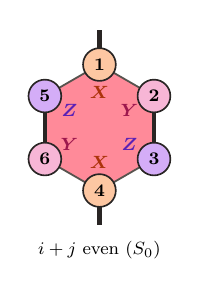
\begin{tikzpicture}[scale=0.8, every node/.style={transform shape}]
\fill[ClassB] (0.000,1.000) -- (0.866,0.500) -- (0.866,-0.500) -- (0.000,-1.000) -- (-0.866,-0.500) -- (-0.866,0.500) -- cycle;
\draw[hexedge] (0.000,1.000) -- (0.866,0.500) -- (0.866,-0.500) -- (0.000,-1.000) -- (-0.866,-0.500) -- (-0.866,0.500) -- cycle;
\draw[linkedge] (0.866,0.500) -- (0.866,-0.500);
\draw[linkedge] (-0.866,0.500) -- (-0.866,-0.500);
\draw[linkedge] (0,1.000) -- (0,1.550);
\draw[linkedge] (0,-1.000) -- (0,-1.550);
\node[qb, fill=PauliX!40, minimum size=5.2mm, font=\footnotesize\bfseries] at (0.000,1.000) {1};
\node[plabel, text=PauliXText, font=\footnotesize] at (0.000,0.550) {$\boldsymbol{X}$};
\node[qb, fill=PauliY!40, minimum size=5.2mm, font=\footnotesize\bfseries] at (0.866,0.500) {2};
\node[plabel, text=PauliYText, font=\footnotesize] at (0.476,0.275) {$\boldsymbol{Y}$};
\node[qb, fill=PauliZ!40, minimum size=5.2mm, font=\footnotesize\bfseries] at (0.866,-0.500) {3};
\node[plabel, text=PauliZText, font=\footnotesize] at (0.476,-0.275) {$\boldsymbol{Z}$};
\node[qb, fill=PauliX!40, minimum size=5.2mm, font=\footnotesize\bfseries] at (0.000,-1.000) {4};
\node[plabel, text=PauliXText, font=\footnotesize] at (0.000,-0.550) {$\boldsymbol{X}$};
\node[qb, fill=PauliY!40, minimum size=5.2mm, font=\footnotesize\bfseries] at (-0.866,-0.500) {6};
\node[plabel, text=PauliYText, font=\footnotesize] at (-0.476,-0.275) {$\boldsymbol{Y}$};
\node[qb, fill=PauliZ!40, minimum size=5.2mm, font=\footnotesize\bfseries] at (-0.866,0.500) {5};
\node[plabel, text=PauliZText, font=\footnotesize] at (-0.476,0.275) {$\boldsymbol{Z}$};
\node[font=\footnotesize, align=center] at (0,-1.950) {$i+j$ even ($S_0$)};
\end{tikzpicture}} & \hspace{1mm}\raisebox{-0.5\height}{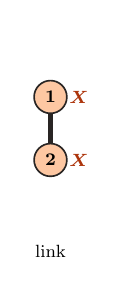
\begin{tikzpicture}[scale=0.8, every node/.style={transform shape}]
\draw[linkedge] (0,0.5) -- (0,-0.5);
\node[qb, fill=PauliX!40, minimum size=5.2mm, font=\footnotesize\bfseries] at (0,0.5) {1};
\node[qb, fill=PauliX!40, minimum size=5.2mm, font=\footnotesize\bfseries] at (0,-0.5) {2};
\node[plabel, text=PauliXText, font=\footnotesize] at (0.45,0.5) {$\boldsymbol{X}$};
\node[plabel, text=PauliXText, font=\footnotesize] at (0.45,-0.5) {$\boldsymbol{X}$};
\node[font=\footnotesize, align=center] at (0,-1.95) {link};
\path (0,1.6) -- (0,-1.6);
\end{tikzpicture}} & \hspace{3mm} & \raisebox{-0.5\height}{
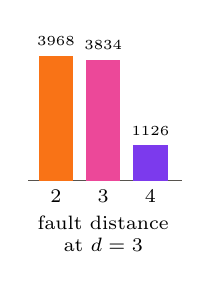
\begin{tikzpicture}
  \draw[InkSoft, line width=0.5pt] (-0.1,0) -- (1.85,0);
  \foreach \x/\h/\n/\c in {0.25/1.587/3968/PauliX, 0.85/1.534/3834/PauliY, 1.45/0.450/1126/LogicalGold}{
    \fill[\c] (\x-0.22,0) rectangle (\x+0.22,\h);
    \node[font=\tiny, above] at (\x,\h) {\n};
  }
  \node[font=\scriptsize, below] at (0.25,0) {2};
  \node[font=\scriptsize, below] at (0.85,0) {3};
  \node[font=\scriptsize, below] at (1.45,0) {4};
  \node[font=\scriptsize, align=center] at (0.85,-0.68) {fault distance\\ at $d=3$};
\end{tikzpicture}}\\
\end{tabular}
\end{tabular}
\end{document}
